% =========================================================
\section{III. Các Vấn Đề Và Thách Thức}

\begin{frame}
\frametitle{Các vấn đề}
   \begin{enumerate}
    \item Liệu bản Saboteur này đã đủ hấp dẫn, có thiếu sót gì có thể bổ sung?
    \item Liệu người thông tin thuộc về một người chơi có bị lộ ra cho các người chơi khác?
    \item Làm sao để số hóa game bài mà vẫn đảm bảo được tính tương tác xã hội?
   \end{enumerate}
\end{frame}

% New Saboteur
% 11
\begin{frame}
\frametitle{Sáng tạo luật chơi mới - Biến thể Saboteur với  ngày đêm}
    \begin{figure}[H]
        \centering
        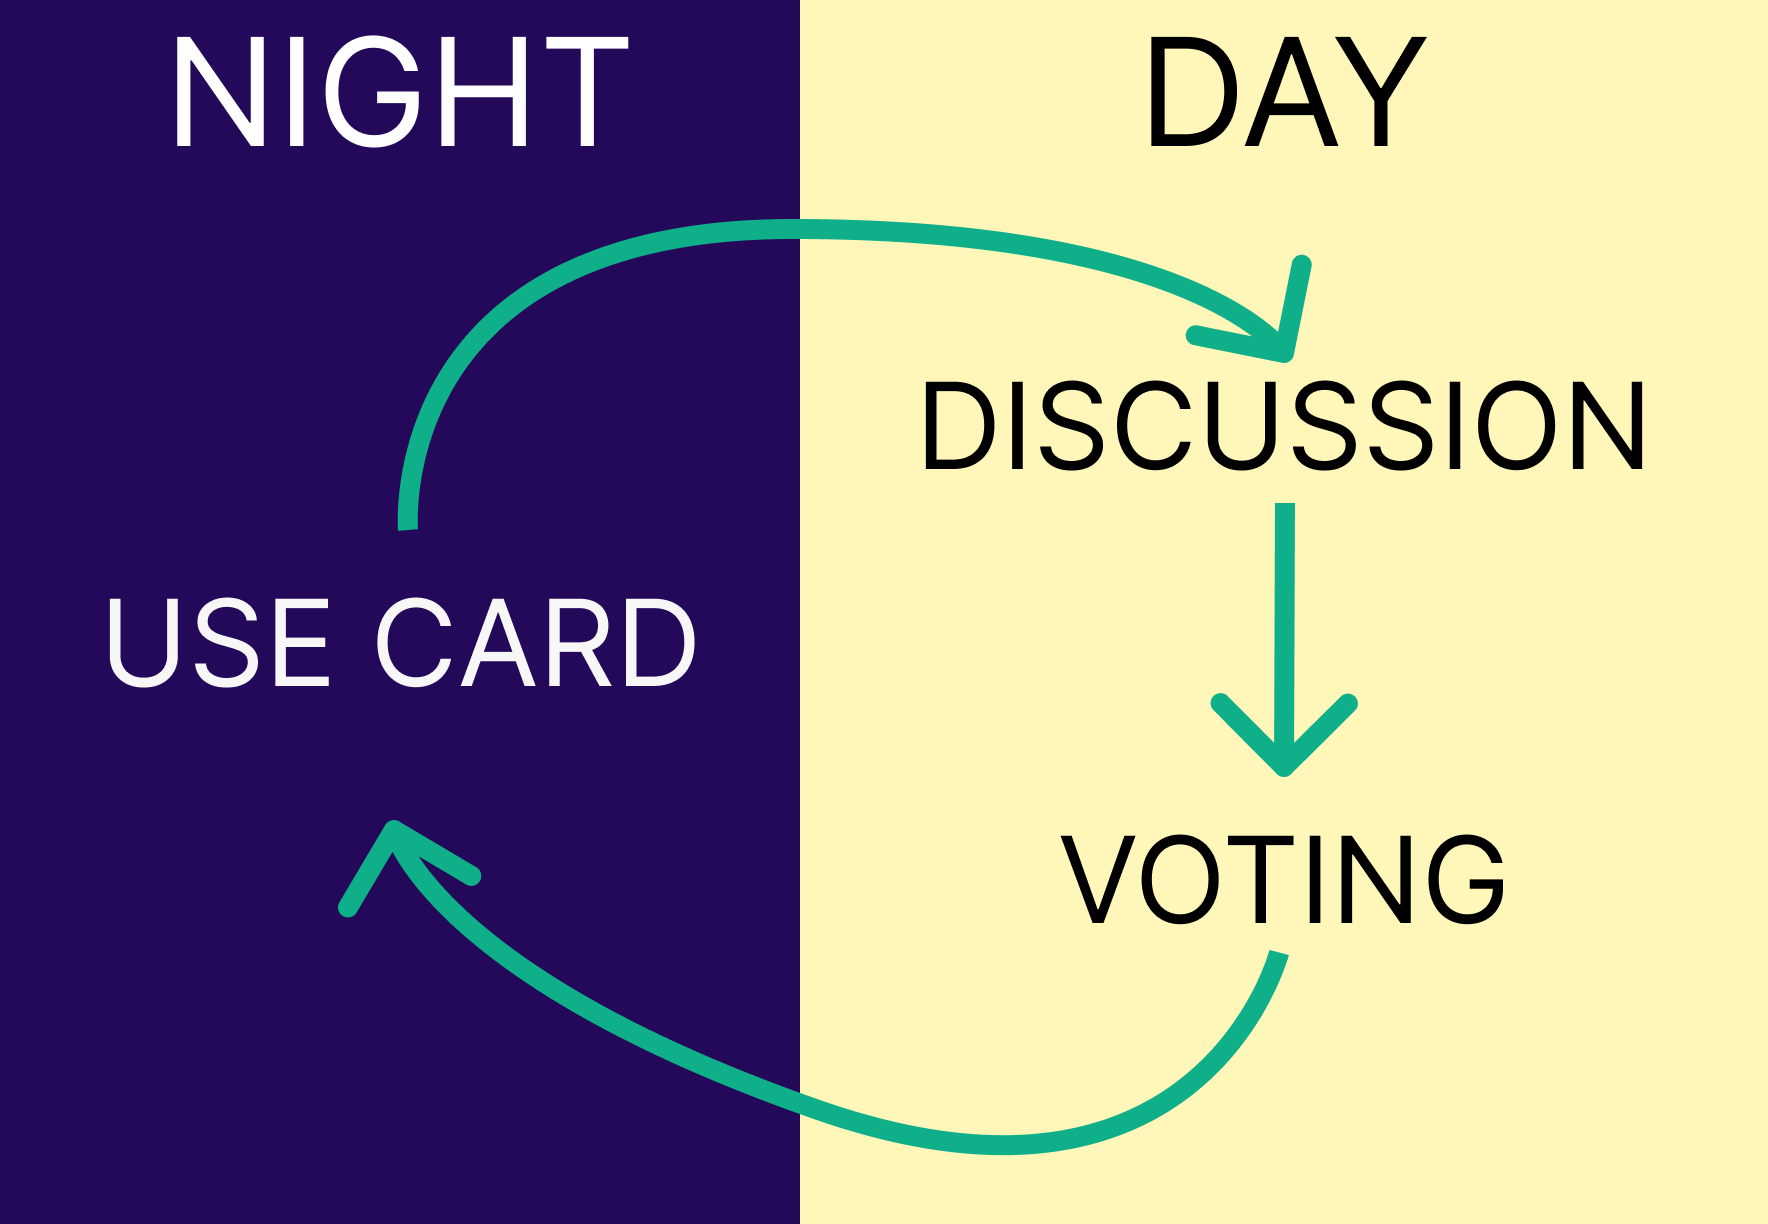
\includegraphics[width=0.5\linewidth]{saboteur/day-night.png}
    \end{figure}
Mỗi round được chia thành hai pha chính: \textbf{Đêm} và \textbf{Ngày}.
\end{frame}

% 12
\begin{frame}
\frametitle{Cấu trúc một round}

\textbf{Đêm (Night Phase):}
\begin{itemize}
    \item Màn hình/bản đồ tối lại, người chơi \textbf{không nhìn thấy bất kỳ thay đổi nào trên bản đồ} ngoại trừ thông tin lượt hiện tại.
    \item Thứ tự lượt chơi trong đêm được \textbf{xếp ngẫu nhiên} (không theo chiều kim đồng hồ như bản gốc).
    \item Mỗi người chơi lần lượt thực hiện lượt:
\begin{itemize}
    \item Bản đồ tạm thời hiện ra cho riêng người đó.
    \item Trong \textbf{15--30 giây} (có thể tùy chỉnh), người chơi thực hiện một trong các hành động quen thuộc như bản gốc.
    \item Bốc 1 lá bài từ chồng bài úp (nếu còn).
    \item Bản đồ lại tối đi với người chơi đó.
\end{itemize}
    \item Khi tất cả người chơi đã hoàn thành lượt trong đêm, pha Đêm kết thúc và chuyển sang pha Ngày.
\end{itemize}

\end{frame}

% 13
\begin{frame}
\frametitle{Cấu trúc một round}
\textbf{Ngày (Day Phase):}
    \begin{itemize}
        \item Bản đồ được chiếu sáng hoàn toàn, mọi người chơi cùng nhìn thấy toàn bộ thay đổi đã xảy ra trong pha Đêm.
        \item Người chơi có \textbf{60 giây} (có thể tùy chỉnh) để \textbf{trò chuyện, tranh luận, biện minh} và đọc vị nhau.
        \item Cuối pha Ngày, thực hiện \textbf{bỏ phiếu}:
        \begin{itemize}
            \item Có thể vote \textbf{skip} hoặc vote một người chơi cụ thể.
            \item Người bị vote nhiều phiếu nhất sẽ \textbf{không được hành động trong pha Đêm tiếp theo}.
        \end{itemize}
    \end{itemize}

\end{frame}

% 15
% \begin{frame}
% \frametitle{Thẻ hành động mới (bổ sung thêm vào bộ bài)}
% \begin{table}[H]
% \centering
% \begin{tabular}{|l|p{7cm}|p{4cm}|}
% \hline
% \textbf{Tên thẻ} & \textbf{Công dụng} & \textbf{Ghi chú} \\ \hline
% 
\includegraphics[width=0.1\linewidth]{saboteur/role-1.png} & Người chơi sẽ có khiên vĩnh viễn có thể đỡ được 1 đòn tấn công phá công cụ (Cart, Shovel, Hat) bởi thẻ Sabotage. & Có thể áp dụng cho bất cứ ai, không tích lũy \\ \hline
% Binoculars & Khi sử dụng thẻ này, người chơi được nhìn thấy toàn bộ bản đồ từ lúc chơi thẻ cho đến hết Đêm hiện tại. & Có thể áp dụng cho bất cứ ai\\ \hline
% Swap Goals & Trong Đêm, tráo vị trí ngẫu nhiên hoặc chỉ định của 3 thẻ Goal (khi chúng vẫn đang úp). & Thay đổi vị trí kho vàng thực sự \\ \hline
% \end{tabular}
% \end{table}
% \end{frame}

\begin{frame}
\frametitle{Thẻ hành động mới}
\begin{columns}
\column{0.33\textwidth}
    \begin{figure}[H]
        \centering
        
\includegraphics[width=0.4\linewidth]{saboteur/Card_Binoculars_S.png}
    \end{figure}
    \begin{itemize}
        \item Nhìn thấy toàn bộ bản đồ từ lúc chơi thẻ cho đến hết \textbf{Đêm} hiện tại.
    \end{itemize}
\column{0.33\textwidth}
    \begin{figure}[H]
        \centering
        
\includegraphics[width=0.4\linewidth]{saboteur/Card_Shield_S.png}
    \end{figure}
    \begin{itemize}
        \item Đỡ được 1 đòn tấn công phá công cụ. Không tích lũy
    \end{itemize}

\column{0.33\textwidth}
    \begin{figure}[H]
        \centering
        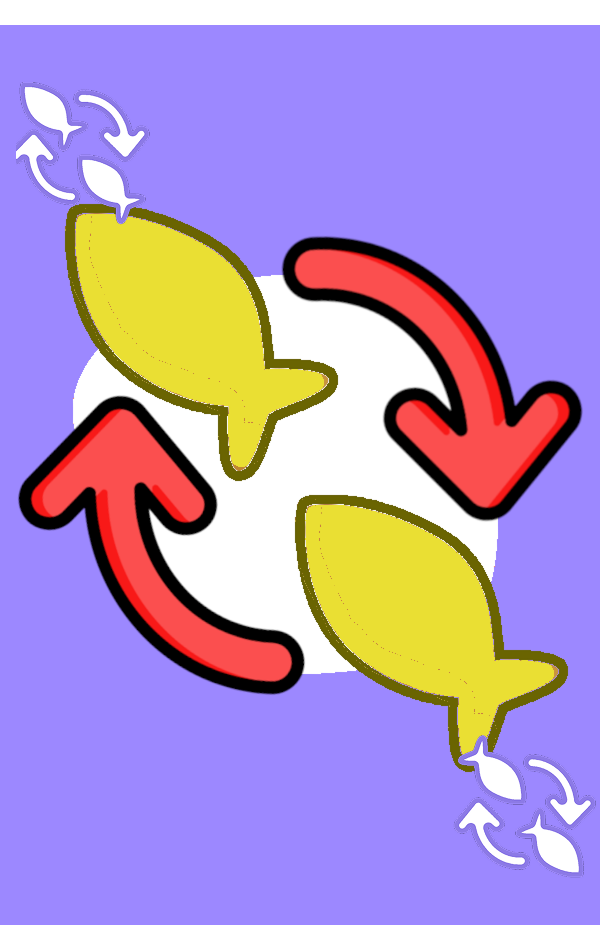
\includegraphics[width=0.4\linewidth]{saboteur/Card_Swap_Goals_S.png}
        % \caption*{Các loại thẻ đường}
    \end{figure}
    \begin{itemize}
        \item Hoán đổi vị trí của 2 trong 3 thẻ Goal (khi chúng vẫn đang úp)
    \end{itemize}
\end{columns}
\end{frame}

% SLIDE 4: Mục Tiêu: Fishy Business
\begin{frame}
\frametitle{Mục Tiêu: Fishy Business}
\begin{columns}
    \column{0.5\textwidth}
    \textbf{1. Hiện thực game}
    \begin{itemize}
        \item Số hóa toàn bộ luật chơi: chia bài, kiểm tra đường đi, tính điểm tự động.
        \item Loại bỏ sự rườm rà của việc thiết lập (setup) thủ công.
    \end{itemize}
    \vspace{0.8em} % Tăng khoảng cách một chút để thoáng bài
    \textbf{2. Mở rộng gameplay}
    \begin{itemize}
        \item Thêm chế độ chơi mới kết hợp giữa saboteur gốc và cơ chế ngày đêm, voting của ma sói.
        \item Thêm các thẻ chức năng để phù hợp với chế độ chơi mới.
    \end{itemize}

    \column{0.5\textwidth}
    \textbf{3. Môi trường 3D}
    \begin{itemize}
        \item Không gian 3D sống động, tối ưu hóa trải nghiệm thị giác.
        \item Người chơi có Avatar, có thể di chuyển và biểu cảm thời gian thực.
    \end{itemize}
    \vspace{0.8em} % Tăng khoảng cách một chút để thoáng bài
    % \textbf{4. Mở rộng môi trường 3D}
    % \begin{itemize}
    %     \item Map mới: battle ship với không gian là trên con thuyền giữa biển khơi, tạo cảm giác tự do, phiêu lưu.
    %     \item Map mới: Playground với không gian là giữa công viên trò chơi, tạo cảm giác vui vẻ, khỏe khắn.
    %     \item Có thể chọn qua lại giữa 3 map khi tạo phòng chơi.
    % \end{itemize}
\end{columns}
\end{frame}


% SLIDE 5: Mục Tiêu: Fishy Business 2
\begin{frame}
\frametitle{Mục Tiêu: Fishy Business}
\begin{columns}
    \column{0.5\textwidth}
    \textbf{4. Multiplayer}
    \begin{itemize}
        \item Kết nối nhiều người chơi thông qua mạng Network.
        \item Tích hợp Voice-Text Chat giúp giao tiếp và "biện minh" trực tiếp.
    \end{itemize}
    \vspace{0.8em} % Tăng khoảng cách một chút để thoáng bài

    \column{0.5\textwidth}
    \vspace{0.8em}
    \textbf{5. Giải trí bổ trợ}
    \begin{itemize}
        \item Giải quyết "thời gian chết" bằng các hoạt động bên lề thú vị.
        \item Chơi nhạc cụ ảo (piano, guitar), thay đổi trang phục linh hoạt.
    \end{itemize}
\end{columns}
\end{frame}
% =========================================================

